\section{Bestemmelse af vandtemperatur i rør}
Da produktet skal overvåge vandspild uden at være indgribende, gøres dette ved at sammenligne overflade temperaturen på vandrøret med temperaturen i rummet. 

\begin{figure}[h!]
  \centering
  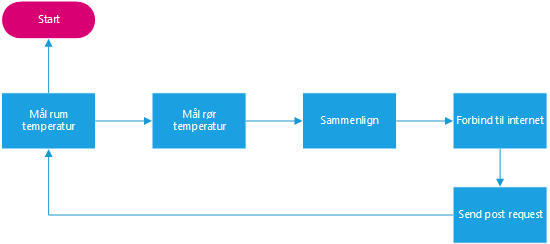
\includegraphics[width=0.7\textwidth]{figures/Fase2software.png}
  \caption{Eksempel på temperaturændringer.}
  \label{tempgraf_eksempel1}
\end{figure}



Figur \ref{tempgraf_eksempel1} viser hvordan temperaturændringerne forekommer hvis det antages at der ingen vandspild er og temperaturen på røret derfor er lig med temperaturen i rummet. I det der tilføres nyt vand til huset ændres rørets temperatur og der vil derfor forekomme temperatursvingninger for at kunne aflæse vandspildet.





\begin{figure}[h!]
  \centering
  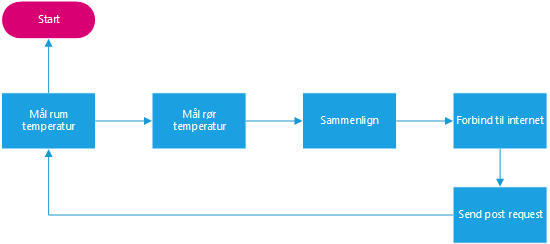
\includegraphics[width=0.7\textwidth]{figures/Fase2software.png}
  \caption{Eksempel på temperaturændringer ved vandspild.}
  \label{tempgraf_eksempelspild}
\end{figure}


Ovenstående figur viser et eksempel på temperaturændringer ved vandspild på et rør. Her ses det hvordan hviletemperaturen på røret aldrig når temperaturen i rummet da vandet aldrig ligger helt stille og derfor tilfører en konstant koldere temperatur.  



    